\documentclass[twocolumn, 10pt]{article}
\usepackage{amsmath}
\usepackage{graphicx}
\usepackage{caption}
\usepackage{float}
\usepackage{multicol}
\usepackage{tikz}
\usepackage{float}
\usepackage[explicit]{titlesec}
\usepackage{geometry}

% Title and Author section formatting like you specifically?
\title{\textbf{Experimental Support for the Conservation of Energy}}
\titlespacing\section{0pt}{12pt plus 4pt minus 2pt}{0pt plus 2pt minus 2pt}
\author{Canada, C., D’Agostino, S., Katz, J., Leung, R.}
\date{December 3rd, 2024} % No date

% Page layout
\setlength{\textwidth}{6.5in}
\setlength{\oddsidemargin}{0in}
\setlength{\evensidemargin}{0in}
\setlength{\topmargin}{-1in}
\setlength{\textheight}{9in}
\geometry{bottom = 0.75in, top = 0.6in}
\setlength{\abovecaptionskip}{1ex}
\setlength{\belowcaptionskip}{1ex}
\setlength{\floatsep}{1ex}
\setlength{\textfloatsep}{1ex}

\begin{document}
\twocolumn[
\begin{@twocolumnfalse}
    \maketitle
    \centering
    \begin{abstract}
		The purpose of this experiment is to investigate the transfer of potential and kinetic energy and confirm the conservation of energy. To investigate, we fired a dart at varying distances using a crossbow. The crossbow launches the dart by releasing an elastic band that pushes the dart along the flight groove of the crossbow, with the dart continuing to move through the air in the direction of the groove. For each distance, at least three trials were conducted. The kinetic energy of the dart was found for each of the distances. The potential energy of the crossbow’s elastic band was also found by measuring various displacements due to various amounts of force applied. The potential and kinetic energy found were then compared. We found that the kinetic energy found was lower than the potential energy found, though this can be attributed to other forces acting on the crossbow and dart, such as friction.


     \end{abstract}
    \vspace{0.5cm}
\end{@twocolumnfalse}
]
\section*{INTRODUCTION}
\hspace{\parindent}	Since the idea was first mathematically developed in the 17th century, energy has proved to be one of the most powerful abstractions in modern physics. Definable as the potential to do work, energy takes many intuitive forms, with the two primary classes being potential and kinetic energy. Potential energy (denoted $U$) is the stored energy of an object due to its position, and is considered by convention to be the opposite of the work done by the conservative forces of a system while an object within it changes position. Work, here, refers to the definite integral (on a displacement interval) of the external force on a system with the differential displacement vector tangent to the system’s trajectory: $W=\int_{x_1}^{x_2} \vec{F}\cdot d\vec{x}$. Kinetic energy is the “active” energy of an object due to its motion, depending on the mass and velocity of the object: $K=\frac{1}{2}mv^2$. Taken together, the two are a system’s mechanical energy, although thermal energy, radiative energy, chemical energy, and many other energy forms contribute to a system’s total energy (the system in question is an arbitrary choice of objects). The conservation of energy then states that the change in the total energy of the system between two arbitrary moments in time is the net energy transferral in and out of the system (see Tipler and Mosca for a more thorough discussion).
\vspace{-5pt}
\begin{gather*}
    \\ E_0 + W + \Delta U_{thermal}= E_F, \text{where}
    \\ E = \sum K + \sum U + \sum U_{thermal} + \sum E_{other}
\end{gather*}
Note that this implies that the total energy of the Universe (or whatever the largest structure is to which energy is a meaningful attribute) always remains constant.

The null hypothesis tested in the experiment discussed in this paper is that $E_0 + W \neq E_F$; that is, that energy is not a conserved quantity in nature. A crossbow was chosen as this experiment’s system of interest in part due it being cost effective and relatively easy to manipulate and measure. The system’s features are also potentially relevant and applicable to various engineering and ballistics problems. For the dart-crossbow system discussed below, the initial energy consists solely of elastic and gravitational potential energy (the latter taken to be 0J for convenience). The final energy of the system (when the dart first leaves the crossbow) is the kinetic energy of the dart, the kinetic energy of the crossbow string, and the thermal energy of the crossbow and dart after they have rubbed against one another during launch.




 \section*{MATERIALS/METHODS}
 \begin{figure}[h]
    \centering
    \textbf{Fig. 1: Crossbow Setup to Find Potential Energy}
    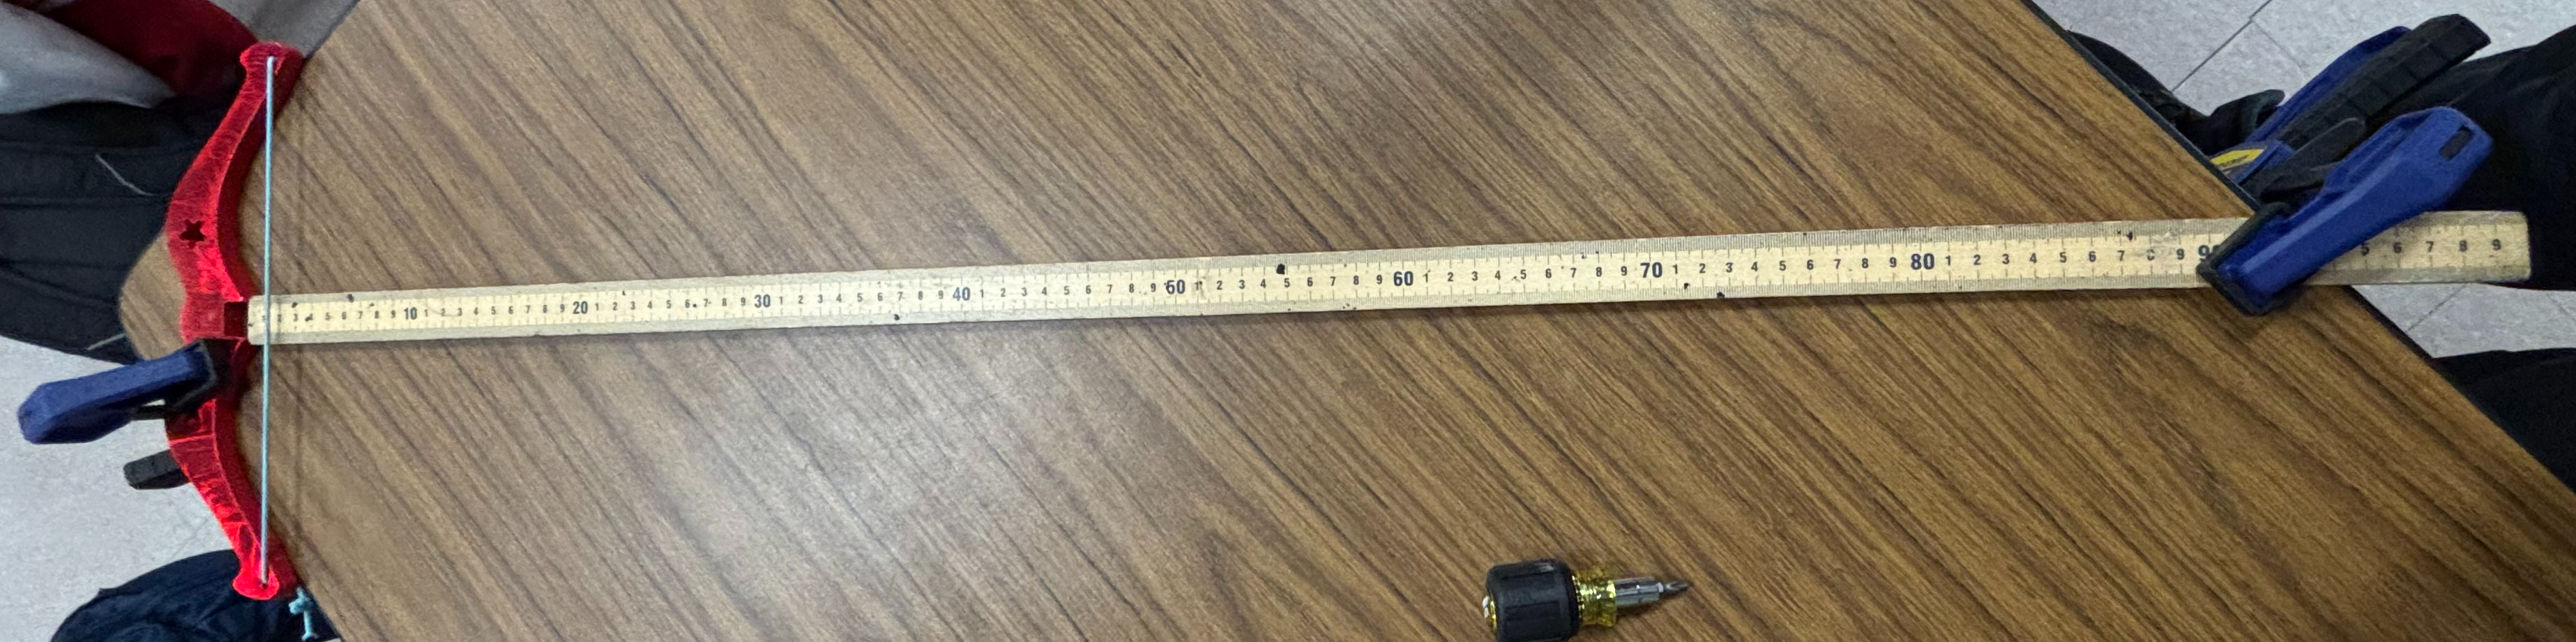
\includegraphics[width=\columnwidth]{PE_Setup.jpg}
\end{figure}
\hspace{\parindent} To measure the potential energy stored in the string of a handmade wooden toy bow by Adventure Awaits!, the meterstick and the unloaded bow were securely clamped to a level surface, perpendicular to one another as shown in Fig. 1. Starting at the 0.16 m mark, which is the distance from the bow's shaft to the string (and thus its equilibrium position), the bowstring was pulled back to every position that required a force of even magnitude (in Newtons) between 0N and 20N. This was done due to the limited precision of the spring scale compared to the meterstick. The force required to pull back the string was measured using a blue 20 Newton spring scale. Two individuals confirmed both the distance the string was pulled and the force required to pull that distance, cross-checking their measurements to ensure accuracy. \par
The total potential energy of the dart-crossbow system when the bow has been drawn 0.1 meters, by the conservation of energy, the work that is required to transform the system to that state from a state of zero energy (i.e. where everything is stationary and the bow is at equilibrium). For the discrete data collected as above, this corresponds to finding the approximate area beneath the curve of the function $\vec{F}(x)$ that the data belongs to. This was done using both a trapezoidal sum on the data and a definite integral of a cubic regression for the data. \par
Secondly, to measure the kinetic energy of the foam projectile (i.e., suction dart) propelled by the bow, the bow and meterstick were set up parallel to one another and positioned securely, ensuring alignment with the testing area and each other. The setup was placed away from the target wall, both vertically and horizontally, with precise measurements taken to establish a shooting distance. Starting at a distance of 2 meters horizontally and 1 meter vertically, the dart was launched toward the wall in three trials, each recorded in slow motion at about 120 frames per second for detailed analysis. This data was collected using the camera off of the Iphone 15 with a 24 MP main camera and a 12 MP ultra wide camera. Frame analysis was done via Apple’s Camera application. The process was then repeated at a horizontal firing distance of 1 meter for four additional trials. Using the slow-motion footage, the initial velocity of the dart was determined by dividing the distance traveled by a given point on the dart (in particular, its backmost end) by the time interval from the moment that point leaves the crossbow to the moment that point stops traveling (i.e., when the dart hits the wall). Since horizontal velocity is independent of vertical influences (i.e., gravity), and the above measurements are taken after the dart has lost contact with the crossbow, this velocity should be almost exactly its initial velocity. Firing distances relatively close to the wall were chosen to minimize the angle at which the dart hits the wall with the horizontal. At greater distances, the dart would begin to measurably point downwards, causing the dart’s extremities to be measured as having travelled farther when in reality its center of mass still has its constant initial velocity. In the calculations, these measurements, combined with the average mass of the darts, were used to calculate their kinetic energy.

 \begin{figure}
    \centering
    \textbf{Fig. 2: Foam Dart Free Body Diagram}
    \includegraphics[width=\columnwidth]{Dart_FBD.jpg}
\end{figure}

 \begin{figure}[h]
    \centering
    \textbf{Fig. 3: Crossbow Free Body Diagram}
    \includegraphics[width=\columnwidth]{CrossbowDiagram.png}
\end{figure}

\section*{RESULTS}
\begin{figure} [h]
    \centering
    \textbf{Fig. 4: Displacement vs. Force of the crossbow string}
    \includegraphics[width=\columnwidth]{Force_VS_Displacement (Cubic).png}
    \textbf{Cubic Regression: $y=61614.9792x^3-6646.49516x^2+243.18397x$ \quad $R^2=0.9848$}
\end{figure}
Taking a trapezoidal Riemann sum of the data from $\Delta x=0\text{m}$ to $\Delta x=0.1\text{m}$ (where $\Delta x$ denotes the displacement of the bow from equilibrium) yields a potential energy fairly close to potential energy calculated via integration of the data’s cubic regression (see p. 306 of Larson et al. for the trapezoidal rule formula):
\vspace{-10pt}
\begin{gather*}
	\\U_s=-W=\int_{0\text{m}}^{0.1\text{m}} \vec{F} \cdot d\vec{x} \approx
\\ \frac{1}{2}\sum_{n=0}^{9} [F(x_n)+F(x_{n+1})]\Delta x_n = 0.512 \text{J}
\\ \approx \int_{0\text{m}}^{0.1\text{m}} y(x) d\vec{x} = 0.541 \text{J}
\end{gather*}

To find the kinetic energy of the dart due to the potential energy of the crossbow (or equivalently, the work done by the crossbow on the dart as it is fired), the dart’s mass and velocity just as it leaves the crossbow must be determined. By taking the average of 19 measurements from a high-precision scale, the mass of the dart in the experiment was about 0.00086 kg. Of the seven trials (three at 2m firing distance and four at 1m), the calculated velocities were 21 m/s for five, 18.6 m/s for one, and 19.4 m/s for one. However (as found during calculations), a time interval uncertainty of $\pm$0.01s results in a velocity uncertainty of up to $\pm$3.1 m/s―$\pm$4.65 m/s. The average of the highest and lowest measured velocities (23.25 m/s and 15.5 m/s, respectively) is about 19.4 m/s, while the average of all measured velocities from all trials (ignoring the uncertainty in each value) is about 20.4 m/s. The kinetic energies due to each are:
\vspace{-10pt}
\begin{gather*}
	\\K = \frac{1}{2}mv_0^2
	\\ K_{extrema} = \frac{1}{2}(0.00086\text{kg})(19.4\text{m/s})^2=0.16\text{J}
	\\ K_{average} = \frac{1}{2}(0.00086\text{kg})(20.4\text{m/s})^2=0.18 \text{J}
\end{gather*}

The percent errors (\% Error) of these with respect to the initial potential energy of the system (calculated by trapezoidal method) are about:
\vspace{-5pt}
\begin{gather*}
	\\ \text{\% Error}_1 = \frac{U_s-K_{extr}}{U_s} = \frac{0.512-0.16}{0.512} = 0.6875
	\\ \text{\% Error}_2 = \frac{U_s-K_{avg}}{U_s} = \frac{0.512-0.18}{0.512} = 0.6484
\end{gather*}

\section*{DISCUSSION}
%\vspace{-13pt}  % 
A comparison of the initial potential energy of the dart-crossbow system and the initial kinetic energy of the dart shows a difference above 60\%, well beyond that solely originating from experimental error (for the purposes of this experiment, about 10\% difference).  These extreme differences, by themselves, would suggest that the experiment’s results are inconclusive at best or that they refute the hypothesis at worst. These results do not, however, conflict with the conservation of energy. The mechanical efficiency of this system is 31.25-35.16\%, which suggests significant energy loss, but which is not unreasonable or uncommon amongst commercially available ballistic devices. In fact, this is consistent with the data collected by Kilaru-et-al, which yielded a similar efficiency of 40.4\%. Several notable causes for an apparent energy loss include the friction between the dart and wooden rail, air drag, and crossbow recoil, all of which result in energy transferral that was not accounted for above. Some rough calculations of these are provided below:
\vspace{-5pt}
\begin{align*}
    \Delta U_{dart/rail} = f_k\Delta x = \mu_kmg\Delta x \approx \\
    (0.3)(0.00086\text{kg})(9.8\frac{\text{m}}{\text{s}^2}) (0.1\text{m}) = 0.00025 \text{J} \\
    \Delta U_{drag} = F_d\Delta x = (\frac{1}{2}C_d\rho v^2 A)(\Delta x) \approx \\
    [\frac{1}{2}(0.9)(1.293\frac{\text{kg}}{\text{m}^3})(20\frac{\text{m}}{\text{s}})(\pi\cdot (0.006\text{m})^2](2\text{m}) \\
    = 0.053 \text{J} \\
    K_{recoil}=\frac{1}{2}m_{crossbow}v_{recoil}^2 = \\
    \frac{1}{2}m_{crossbow}(\frac{m_{dart}}{m_{crossbow}}v_{dart})^2\approx \\
    (0.5)(0.2\text{kg})(\frac{0.00086\text{kg}}{0.2\text{kg}} \cdot 20\frac{\text{m}}{\text{s}})^2 = 0.00081 \text{J}
\end{align*}

%One source of unaccounted-for energy is the friction between the dart and rail as well as the string and rail. A quick, rough calculation of the approximate loss of energy due to friction reveals it to be about 5\% of the system's initial energy: $\Delta U_{thermal} = f_k\Delta x = \mu_kmg\Delta x \approx (0.3)(0.00086\text{kg})(9.8\frac{\text{m}}{\text{s}^2} (0.1\text{m}) = 0.00025 \text{J}$. Similarly, the crossbow's recoil can be assessed by treating the dart's launch as an explosion, taking about 0.1\% of the initial energy: $K_{recoil}=\frac{1}{2}m_{crossbow}v_{recoil}^2 = \frac{1}{2}m_{crossbow}(\frac{m_{dart}}{m_{crossbow}}v_{dart})^2\approx (0.5)(0.2\text{kg})(\frac{0.00086\text{kg}}{0.2\text{kg}} \cdot 20\frac{\text{m}}{\text{s}})^2 = 0.00081 \text{J}$. $C_d = 0.013\text{m}$.

Additionally, if the string isn't 100\% resilient, some energy could be lost to the strain placed on it. A potential source of error is any imprecision of the equipment used. Instead of relying on manual calculations, technology such as motion sensors could have been used to more accurately measure the speeds of projectiles, leading to a better determination of the kinetic energy.

Energy-analysis is advantageous since energy is a scalar as opposed to a vector, whose components depend on coordinate orientation. If force, mass, and velocity can be shown to give rise to a conserved quantity like mechanical energy, this can then provide valuable insight into the behavior of numerous systems, from simple projectiles to complex engines, by offering a vastly more straightforward method of finding the system's dynamical laws.
\vspace{-8pt}

\section*{ACKNOWLEDGMENTS} 

Thank you to the chief editor of the Journal of Science and Engineering, Dr. Evangelista, for his continued support.

\section*{Resources/Bibliography}
[1] P.A. Tipler, and G. Mosca, Physics for Scientists and Engineers (Macmillan Higher Education, 2007).
[2] Larson, Hostetler, and Edwards, Calculus, Fifth Edition (D.C. Heath and Company, 1994)
[3] Gut, Kilaru, and Swami, Efficiency of Conversion between Elastic Potential Energy in a Nerf Crossbow to Kinetic Energy in a Nerf Dart (Journal of Science and Engineering, 2025)

\end{document}


